\chapter{OPIS ROZWIĄZANIA}
\label{chapter:opis_rozwiazania}

\section{Architektura systemu}

System składa się z pięciu głównych komponentów: nadajników BLE (ang. \textit{BLE beacon}), aplikacji mobilnej, systemu Wit.ai, serwera oraz bazy danych. Grafikę przedstawiającą architekturę systemu można zobaczyć na rysunku \ref{fig:architecture}.

\begin{figure}[H]
    \centering
    \includesvg[width=\textwidth]{images/architecture.svg}
    \caption{Architektura systemu.}
    \label{fig:architecture}
\end{figure}

Aplikacja mobilna jest odpowiedzialna za odbieranie oraz przetwarzanie sygnału z nadajników. Jej zadaniem jest również interakcja z użytkownikiem i wysyłanie zapytań do serwera. Serwer przetwarza żądania użytkownika, wysyła zapytania do API (ang. \textit{Application Programming Interface}) serwisu Wit.ai, oraz komunikuje się z bazą danych. Baza danych przechowuje dane i modyfikuje lub udostępnia je na żadanie serwera. Komunikacja między aplikacją mobilną a serwerem odbywa się za pomocą protokołu HTTP. Serwer jest odpowiedzialny za przetwarzanie żądań użytkownika, a także za komunikację z bazą danych. Baza danych przechowuje dane o produktach, użytkownikach, koszykach, sklepach itp.

\section{Baza danych}

\subsection{Opis bazy danych}

Baza danych została zaimplementowana w PostgreSQL. Wybór tej bazy danych wynika z jej wszechstronności, wydajności oraz możliwości łatwego skalowania. 

PostgreSQL to obiektowo-relacyjny system zarządzania bazami danych (ang. ORDBMS \textit{Object-Relational Database Management System}), którego rozwój rozpoczął się już w 1977 roku. Jego korzenie sięgają projektu o nazwie Ingres, realizowanego na Uniwersytecie Kalifornijskim w Berkeley.
Uznawany jest za jeden z najbardziej zaawansowanych systemów baz danych o otwartym kodzie źródłowym na świecie. Oferuje wiele funkcji, które do tej pory były kojarzone głównie z komercyjnymi rozwiązaniami klasy enterprise. \cite{worsley2002practical}

Baza danych przechowuje informacje o produktach, użytkownikach, koszykach oraz sklepach. Schemat bazy danych przedstawia rysunek \ref{fig:database}.

Struktura bazy danych została zaprojektowana w sposób modularny, umożliwiając efektywne zarządzanie danymi dotyczącymi sklepów, użytkowników oraz produktów. Główną tabelą bazy danych jest tabela \textit{stores}, która przechowuje informacje o sklepach, takie jak nazwa, współrzędne geograficzne oraz miasto. Związek tej tabeli z tabelą \textit{sections} umożliwia podział sklepów na sekcje, które z kolei są przypisane do tabeli \textit{categories}, zawierającej dane o kategoriach produktów.

Produkty są przechowywane w tabeli \textit{products}, gdzie każdy rekord zawiera szczegóły takie jak nazwa, opis, cena, dostępność, ilość oraz jednostka miary, przechowywana w tabeli \textit{units}. Relacje między tabelami \textit{categories} i \textit{p}roducts pozwalają na przypisanie każdego produktu do konkretnej kategorii, co ułatwia organizację i wyszukiwanie danych.

Użytkownicy systemu są reprezentowani w tabeli \textit{users}, gdzie zapisywane są ich dane personalne, takie jak imię, nazwisko, adres e-mail oraz zaszyfrowane hasło. Każdy użytkownik może posiadać wiele koszyków zakupowych, co jest odzwierciedlone w tabeli \textit{carts}, przechowującej informacje o koszykach, takie jak data utworzenia i powiązanie z użytkownikiem. 
Szczegóły dotyczące zawartości koszyków są zapisane w tabeli \textit{cart\_items}, która łączy produkty z koszykami i zawiera informacje o liczbie sztuk danego produktu.

Relacje pomiędzy tabelami są realizowane za pomocą kluczy obcych, z zastosowaniem reguły ON DELETE CASCADE, co zapewnia integralność danych oraz automatyczne usuwanie powiązanych rekordów w przypadku usunięcia danych z tabel nadrzędnych. Taka organizacja umożliwia łatwe skalowanie bazy danych oraz wspiera utrzymanie spójności danych w systemie.

\begin{figure}[H]
    \includesvg[width=\textwidth]{images/database.svg}
    \caption{Schemat bazy danych.}
    \label{fig:database}
\end{figure}

\subsection{Szczegółowy opis tabel}

\subsubsection{Tabela stores}
\begin{itemize}
\item store\_id - SERIAL PRIMARY KEY: Unikalny identyfikator każdego sklepu.
\item store\_name - VARCHAR(255) NOT NULL: Nazwa sklepu.
\item latitude - VARCHAR(255) NOT NULL: Szerokość geograficzna określająca położenie sklepu.
\item longitude - VARCHAR(255) NOT NULL: Długość geograficzna określająca położenie sklepu.
\item city - VARCHAR(255) NOT NULL: Miasto, w którym znajduje się sklep.
\end{itemize}

\subsubsection{Tabela sections}
\begin{itemize}
\item section\_id - SERIAL PRIMARY KEY: Unikalny identyfikator sekcji sklepu.
\item section\_name - VARCHAR(255) NOT NULL: Nazwa sekcji w sklepie.
\item store\_id - INT REFERENCES stores(store\_id) ON DELETE CASCADE: Klucz obcy wskazujący sklep, do którego należy sekcja.
\end{itemize}

\subsubsection{Tabela categories}
\begin{itemize}
\item category\_id - SERIAL PRIMARY KEY: Unikalny identyfikator kategorii.
\item category\_name - VARCHAR(255) NOT NULL: Nazwa kategorii produktów.
\item section\_id - INT REFERENCES sections(section\_id) ON DELETE CASCADE: Klucz obcy wskazujący sekcję, do której przypisana jest kategoria.
\end{itemize}

\subsubsection{Tabela units}
\begin{itemize}
\item unit\_id - SERIAL PRIMARY KEY: Unikalny identyfikator jednostki miary.
\item unit\_name - VARCHAR(50) NOT NULL: Pełna nazwa jednostki miary (np. “kilogram”).
\item unit\_symbol - VARCHAR(10) NOT NULL: Skrót jednostki miary (np. “kg”).
\end{itemize}

\subsubsection{Tabela products}
\begin{itemize}
\item product\_id - SERIAL PRIMARY KEY: Unikalny identyfikator produktu.
\item name - VARCHAR(255) NOT NULL: Nazwa produktu.
\item description - TEXT: Opis produktu.
\item price - DECIMAL(10,2) NOT NULL: Cena produktu w formacie dziesiętnym (np. 123.45).
\item category\_id - INT REFERENCES categories(category\_id) ON DELETE CASCADE: Klucz obcy wskazujący kategorię, do której należy produkt.
\item availability - VARCHAR(50) NOT NULL: Status dostępności produktu (np. “w magazynie”).
\item amount - DECIMAL(10,2) NOT NULL: Ilość dostępna w magazynie.
\item unit\_id - INT REFERENCES units(unit\_id) ON DELETE CASCADE: Klucz obcy wskazujący jednostkę miary produktu.
\end{itemize}

\subsubsection{Tabela users}
\begin{itemize}
\item user\_id - SERIAL PRIMARY KEY: Unikalny identyfikator użytkownika.
\item email - VARCHAR(255) UNIQUE NOT NULL: Adres e-mail użytkownika.
\item password - VARCHAR(255) NOT NULL: Hasło użytkownika (w formie zaszyfrowanej).
\item first\_name - VARCHAR(50) NOT NULL: Imię użytkownika.
\item last\_name - VARCHAR(50) NOT NULL: Nazwisko użytkownika.
\end{itemize}

\subsubsection{Tabela carts}
\begin{itemize}
\item cart\_id - SERIAL PRIMARY KEY: Unikalny identyfikator koszyka.
\item user\_id - INT REFERENCES users(user\_id) ON DELETE CASCADE: Klucz obcy wskazujący użytkownika, do którego należy koszyk.
\item creation\_date - TIMESTAMP DEFAULT CURRENT\_TIMESTAMP: Data i czas utworzenia koszyka.
\end{itemize}

\subsubsection{Tabela cart\_items}
\begin{itemize}
\item cart\_item\_id - SERIAL PRIMARY KEY: Unikalny identyfikator pozycji w koszyku.
\item cart\_id - INT REFERENCES carts(cart\_id) ON DELETE CASCADE: Klucz obcy wskazujący koszyk, do którego należy pozycja.
\item product\_id - INT REFERENCES products(product\_id) ON DELETE CASCADE: Klucz obcy wskazujący produkt dodany do koszyka.
\item quantity - INT NOT NULL: Liczba sztuk danego produktu w koszyku.
\end{itemize}

tekst

\section{Interfejs użytkownika}

\subsection{Opis dostępnych widoków}

\subsubsection{Strona tytułowa}

\begin{center}
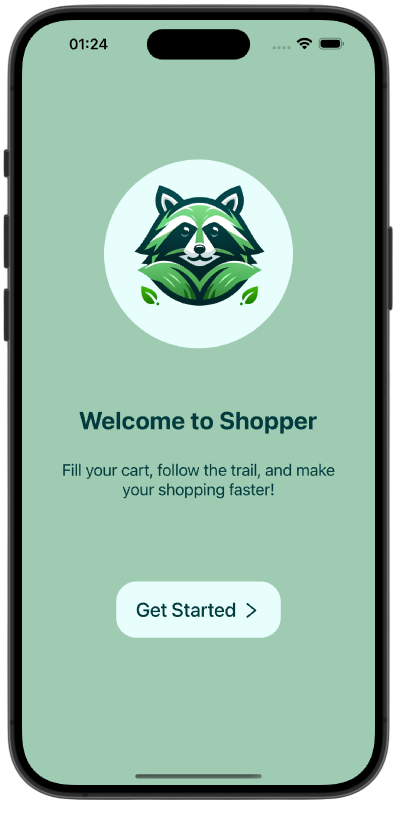
\includegraphics[width=0.4\textwidth]{images/front/home_page.png}
\end{center}

Strona tytułowa aplikacji pełni funkcję ekranu startowego, witając użytkownika logiem oraz hasłem zachęcającym do korzystania z aplikacji. Ponadto, widnieje  na niej przycisk "Get Started", który umożliwia przejście do kolejnych widoków. Jeśli użytkownik był zalogowany, w ciągu ostatnich 7 dni, aplikacja przekierowuje go do widoku logowania. W przeciwnym wypadku trafia on do ekranu profilu. Całość utrzymana jest w przyjaznej stylistyce, z dominującym odcieniem zieleni oraz spójną paletą kolorów, wygenerowaną przez narzędzie DALL·E 3 od OpenAI.

\begin{center}
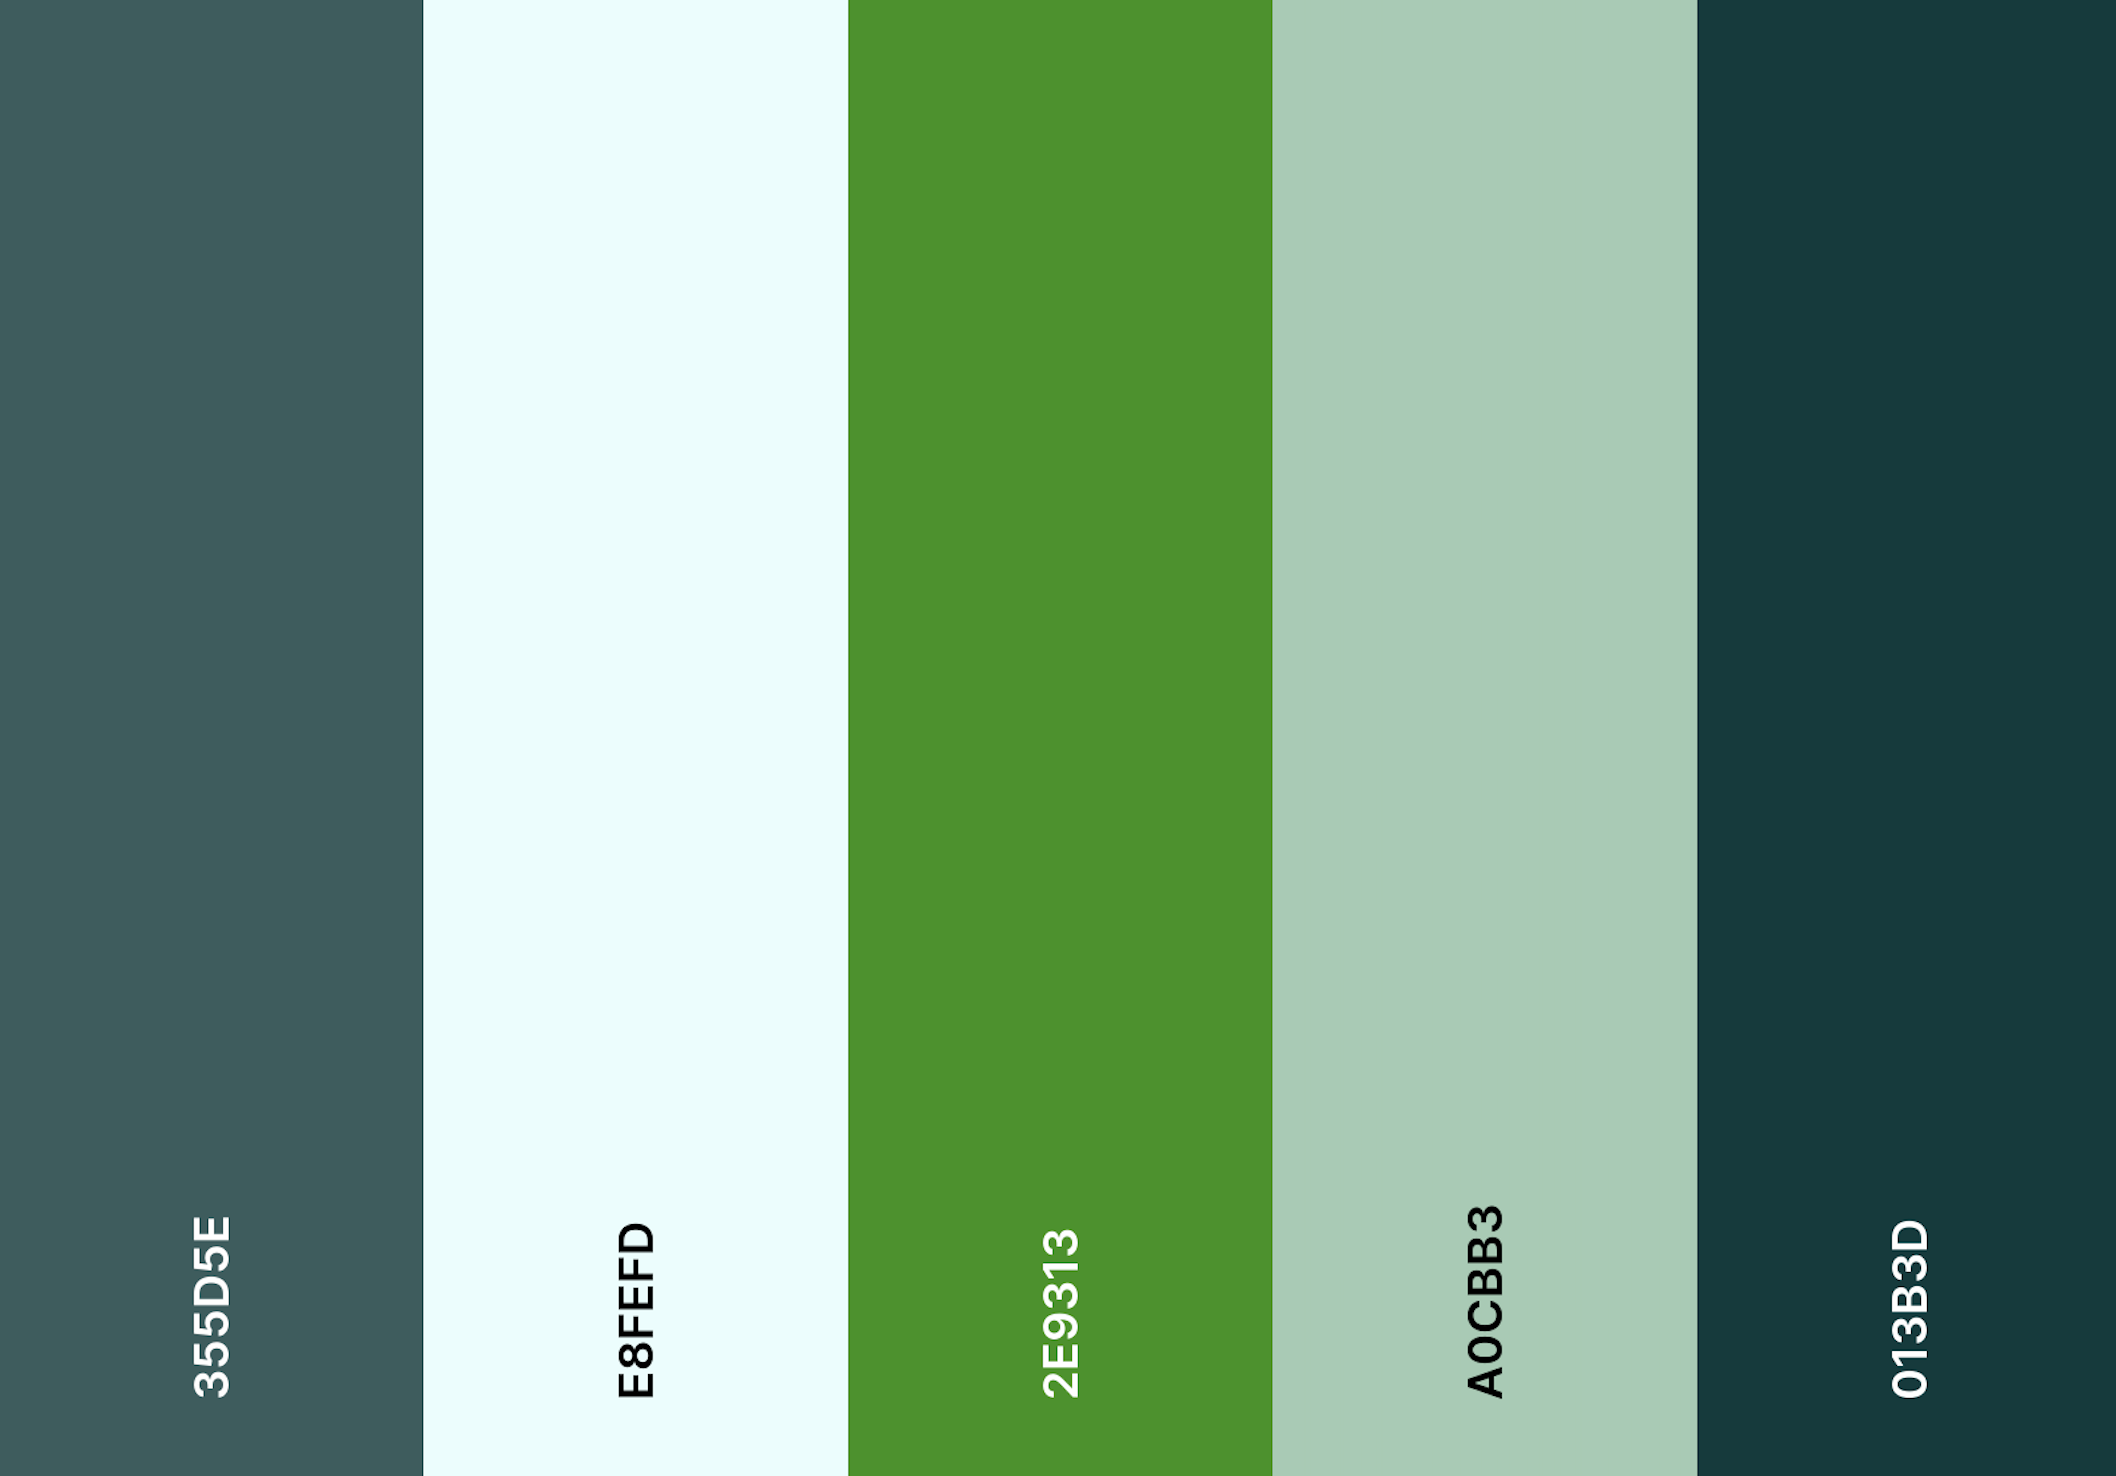
\includegraphics[width=0.6\textwidth]{images/front/theme.png}
\end{center}

\subsubsection{Ekran logowania}

text

\subsection{Szczegółowe omówienie implementacji}

\subsubsection{Strona tytułowa}


\section{Serwer aplikacji}
Serwer jest odpowiedzialny za przetwarzanie żądań użytkownika, a także za komunikację z bazą danych. Został zaimplementowany w języku JavaScript przy użyciu platformy Node.js oraz struktury (ang. \textit{framework}) Express.js. Node.js pozwala na uruchamianie JavaScript po stronie serwera, co umożliwia tworzenie wydajnych i skalowalnych aplikacji. Express.js, będący minimalistycznym frameworkiem działającym na Node.js, upraszcza proces budowy aplikacji internetowych. Serwer nasłuchuje na zapytania HTTP, przetwarza je i zwraca odpowiedź, a do komunikacji z bazą danych PostgreSQL wykorzystuje odpowiednie moduły Node.js.


\subsection{JavaScript}
JavaScript jest podstawowym językiem programowania w sieci Web. Zdecydowana większość współczesnych stron internetowych wykorzystuje JavaScript, a wszystkie nowoczesne przeglądarki internetowe — zarówno na komputerach stacjonarnych, konsolach do gier, tabletach, jak i smartfonach — posiadają wbudowane interpretery tego języka. Dzięki temu JavaScript stał się najbardziej wszechobecnym językiem programowania w historii. Wraz z HTML, odpowiadającym za treść stron, oraz CSS, definiującym ich wygląd, JavaScript stanowi podstawowy zestaw technologii, które każdy programista webowy musi opanować, aby określać zachowanie stron internetowych. \cite{flanagan2011javascript}


\subsection{Node.js}
Node.js umożliwia programistom wykorzystywanie JavaScript po stronie serwera, co pozwala na tworzenie aplikacji full-stack przy użyciu jednego języka. Dzięki architekturze wspierającej asynchroniczne i nieblokujące operacje I/O świetnie sprawdza się w obsłudze wielu jednoczesnych połączeń. \cite{peters2017building}

Dzięki architekturze opartej na zdarzeniach oraz jednowątkowemu modelowi działania, Node.js idealnie nadaje się do tworzenia aplikacji czasu rzeczywistego, takich jak czaty, narzędzia do współpracy czy usługi streamingowe. \cite{peters2017building}

\subsection{Express.js}
Express.js to minimalistyczny framework dla Node.js, który pozwala na szybkie tworzenie aplikacji internetowych. Dzięki swojej prostocie i elastyczności jest jednym z najpopularniejszych frameworków dla Node.js.

Framework Express.js umożliwia dynamiczny routing, pozwalając programistom na definiowanie wzorców URL i przypisywanie ich do określonej logiki aplikacji. Taka elastyczność ułatwia zarządzanie złożonymi strukturami aplikacji poprzez wiązanie punktów końcowych z odpowiednimi kontrolerami. \cite{peters2017building}
